\chapter[Referencial Teórico]{Referencial Teórico}

\section{Engenharia de Requisitos}

O conjunto de tarefas e técnicas utilizadas para promover o entendimento dos requisitos é denominado Engenharia de Requisitos. Na visão do desenvolvimento de software, pode ser vista como uma fase importante de Engenharia de Software que se inicia na atividade de comunicação e continua até a entrega do produto de software, sendo adaptada de acordo com as necessidades do processo de desenvolvimento de software, do produto e dos \textit{stakeholders} \cite{pressman2011engenharia}.

A Engenharia de requisitos abrange sete fases distintas: concepção, levantamento, elaboração, negociação, especificação, verificação e validação \cite{pressman2011engenharia}. De acordo com \cite{kotonya1998requirements} durante a execução das atividades das fases da Engenharia de Requisitos alguns problemas são relatados como: (i) Os requisitos não refletem as reais necessidades do cliente de acordo com o sistema a ser desenvolvido; (ii) Os requisitos são inconsistentes e/ou incompletos; (iii) É complexo a realização de alguma mudança no requisito, logo após terem sido acordado pelas partes; (iv) comumente o requisito é interpretado de maneira errada entre a equipe de desenvolvimento de software e o cliente.  

A maioria dos modelos dentro da engenharia de requisitos, não possuíam um tratamento adequado para tratar os atributos de qualidade, logo o tratamento desses atributos de qualidade tem sido um foco chave de trabalhos na área da Engenharia de Requisitos Orientada a Meta \cite{chung2012non}. Entretanto neste trabalho é abordado o NFR \textit{framework} que trata os requisitos não funcionais em um nível mais alto de abstração, tanto para o problema quanto para a solução. 

\subsection{Engenharia de Requisitos Orientada a Meta}

Os requisitos de software muitas vezes são elicitados, modelados e analisados como metas ao qual os \textit{stakeholders} querem alcançar \cite{van2001goal}. O termo \textit{Goal-Oriented Requirements Engineering} (GORE) surgiu nas duas últimas décadas. Tipicamente as metas são elicitadas e conceituadas  em termos de alguma forma de modelo. Os modelos de metas têm sido utilizados como um meio eficaz para capturar as interações e os compromissos entre os requisitos \cite{letier2002deriving}. As metas também podem contemplar diferentes tipos de interesses: interesses funcionais associados ao serviço que deverá ser prestado e interesses não funcionais associados a qualidade do serviço (precisão, desempenho, segurança) \cite{van2001goal}.
 
Para auxiliar no entendimento das metas podem ser realizados as seguintes perguntas "por que?", "como?", "de que outra forma?"\cite{van2001goal}. Onde o "por que?" auxilia na compreensão de objetivos superiores e logo se um requisito não é considerado se não possuir uma contribuição para um objetivo superior; O "Como?" ajuda a entender as metas em níveis inferiores\cite{yu1998goal}; E "de que outra forma?" ajuda no processo de identificação de possíveis alternativas para o atendimento de metas superiores \cite{van2001goal}.  

\subsection{Requisitos Não-Funcionais}

Na literatura pode ser encontrada uma infinidade de definições os NFRs, mas normalmente vem sendo referenciados em termos que terminam com as palavras "-ilidades" ou "-idades", mas também existem outros termos que referenciam requisitos não funcionais como por exemplo, desempenho, coerência, segurança, etc \cite{chung2012non}. Na área de arquitetura de software um termo frequentemente encontrado é atributos de qualidade\cite{barbacci1995quality}.

Os impactos diretos no tempo de execução, design do sistema e na experiência do usuário são diretamente ligados aos atributos de qualidade, o conjunto de atributos de qualidade representam as áreas de interesse que possuem grande impacto em seus níveis e camadas. Alguns atributos possuem impacto geral ao design do sistema (Exemplo: Suportabilidade) e outros atuam em problemas mais específicos (Exemplo: Usabilidade), é somente então quando a aplicação de software a ser desenvolvida atende uma combinação desejada desses atributos que indicam o sucesso do design e a qualidade geral do aplicativo de software \cite{microsoft2009}.

\section{NFR Framework}

O NFR Framework é um modelo intencional que ajuda os desenvolvedores  a  lidar com requisitos não-funcionais através de grafos, que podem ser visualizados na forma interativa e incremental, da análise e revisão de um \textit{Softgoal Interdependency Graphs} - SIGs. O framework possui uma estrutura orientada por processo e pode ser utilizado como complemento nas abordagens tradicionais orientada a produto. Dando suporte aos desenvolvedores em seus \textit{softgoals} e os \textit{tradeoffs} (situações onde existem conflitos de escolha). Diante da complexidade de tratar os RNFs enfrentada pelos desenvolvedores em projetos de software a o tratamento dos RNFs	pode ser facilitado através do uso de catálogos de conhecimento para os RNFs \cite{chung2012non}. 


É através do SIGs que é mantido todo o registro das decisões tomada durante todo o processo de desenvolvimento do software e as decisões de design em forma gráfica e consisa, este registro gráfico possibilita aos desenvolvedores acompanhar as decisões sobre os requisitos não funcionais, as alternativas associadas  ao requisito, decisões e as razões pelas quais as decisões foram tomadas. É no SIGs que surge os principais conceitos do NFR Framework. como \textit{softgoals} que são os principais requisitos e são apresentados como uma nuvem na parte superior do grafo, esses \textit{softgoals} podem ser conectados através de links de interdependência com outros \textit{softgoals} \cite{chung2012non}.

O NFR framework é composto por cinco componentes, sendo eles: Sofgoals, Interdependências, Procedimento de avaliação, Métodos e as Correlações \cite{chung2012non}. Esses elementos serão detalhados abaixo, bem como suas representações gráficas. 

\begin{itemize}
	\item \textit{Softgoals}
	
	É a unidade básica utilizada na representação dos RNFs, podendo assumir as naturezas: Subjetiva, pois o RNF pode variar de acordo com o julgamento de cada pessoa; Relativa, pois o RNF pode depender de algum tipo de relação com algum outro RNF. Existem três tipos de \textit{softgoals}: (i) \textit{Softgoals} de RNFs, que representam os requisitos não funcionais para serem satisfeitos; (ii) \textit{Operationalizing softgoals}, basicamente são as técnicas de desenvolvimento que ajudam a satisfazer o requisito não funcional, elas podem aparecer como uma operação, representação de dados, restrição ou atribuição de um agente externo a uma tarefa; (iii) \textit{Claim sofgoals}, é o tipo que ajuda para a tomada de decisões. A representação gráfica dos tipos de \textit{softgoals} pode ser consultada na figura \ref{fig01}.
	
	\begin{figure}[h]
		\centering
		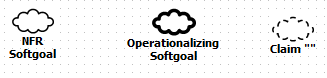
\includegraphics[keepaspectratio=true,scale=0.9]{figuras/tiposDeSoftgoals.png}
		\caption{Representação gráfica dos tipos de \textit{softgoals}.}
		\label{fig01}
	\end{figure} 

	Os \textit{softgoals} também trabalham com o conceito de labels, possibilitando o entendimento das decisões tomadas, ficando assim registradas no desenho do gráfico SIG de acordo com  a figura \ref{fig02} . Os tipos de labels são: satisfeita, negada, fracamente satisfeita, fracamente negada, crítica e indecidida.
	

	\begin{figure}[h]
		\centering
		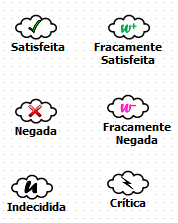
\includegraphics[keepaspectratio=true,scale=0.9]{figuras/labelsSoftgoals.png}
		\caption{Representação gráfica das labels de \textit{softgoals}.}
		\label{fig02}
	\end{figure} 

	\item Interdependências
	
	É o componente responsável por estabelecer as inter-relações entre os \textit{softgoals}. As interdependências que fazem o registro do refinamento dos \textit{softgoals} em \textit{softgoals} mais específicos (filhos), e suas contribuições para a satisfazer o \textit{softgoal} mais genêrico (pai). Os tipos de contribuições são: AND, OR, ++, --, +, -, S+, S-. 
	
	\begin{table}[h!]
		\centering
		\caption{Tipos de contribuições}
		\label{tiposDeContribuições}
		\begin{tabular}{|l|l|}
			\hline
			\textbf{Símbolo} & \textbf{Descrição} \\ \hline
			\multirow{2}{*}{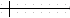
\includegraphics[scale=0.9]{figuras/And.png}} & \multirow{2}{*}{AND: Se todos os filhos são satisfeitos o pai também será satisfeito.} \\
			&  \\ \hline
			\multirow{2}{*}{\includegraphics[scale=0.9]{figuras/OR.png}} & \multirow{2}{*}{OR: Se qualquer filho é satisfeito o pai também será satisfeito.} \\
			&  \\ \hline
			\multirow{2}{*}{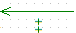
\includegraphics[scale=0.9]{figuras/Make.png}} & \multirow{2}{*}{\begin{tabular}[c]{@{}l@{}}MAKE: Pode ser tratado de forma semelhante ao AND, pois se \\ o filho for satisfeito o pai pode ser satisfeito.\end{tabular}} \\
			&  \\ \hline
			\multirow{2}{*}{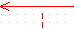
\includegraphics[scale=0.9]{figuras/Break.png}} & \multirow{2}{*}{\begin{tabular}[c]{@{}l@{}}BREAK: Fornece apoio negativo, pois se o filho é satisfeito o \\ pai pode ser negado.\end{tabular}} \\
			&  \\ \hline
			\multirow{2}{*}{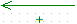
\includegraphics[scale=0.9]{figuras/Help.png}} & \multirow{2}{*}{HELP: Se todos os filhos são satisfeitos o pai também será satisfeito.} \\
			&  \\ \hline
			\multirow{2}{*}{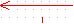
\includegraphics[scale=0.9]{figuras/Hurt.png}} & \multirow{2}{*}{HURT: Se todos os filhos são satisfeitos o pai também será satisfeito.} \\
			&  \\ \hline
			\multirow{2}{*}{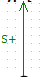
\includegraphics[scale=0.9]{figuras/SomeMais.png}} & \multirow{2}{*}{SOME+: Representa a existência de alguma contribuição positiva.} \\
			&  \\ \hline
			\multirow{2}{*}{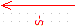
\includegraphics[scale=0.9]{figuras/SomeMenos.png}} & \multirow{2}{*}{SOME-: Representa a existência de alguma contribuição negativa.} \\
			&  \\ \hline
		\end{tabular}
	\end{table}
	
	\item Métodos
	
	É o componente responsável por fornecer aos desenvolvedores catálogos com as técnicas de desenvolvimento, os métodos basicamente são refinados de \textit{softgoals} em outros \textit{softgoals}
	
	\item Correlações
	
	Os \textit{softgoals} possuem possíveis relações tanto positivas quanto negativas, as correlações são catálogos para poder inferir nessas possíveis relações. 
\end{itemize}

\subsection{i*}

\subsection{FURPS}


\section{Arquitetura de Software}

\subsection{MVC - Model-View-Controller}

\chapter{Metodologia}

\subsection{Classificação da Pesquisa}